% Master inclusion file for all Dimer plates
\section{The Complete Catalogue of 295 Dimers}
\label{sec:dimers-catalogue}

Each vertical bi-cartouche contains an affine dimer $\{O_a, O_b\}$ of shape $z_4^4$ on $\mathbb{Z}_{16}$, paired under the Galois multiplier $\mu_3 \colon x \mapsto 3x$ (top to bottom). The top mosaic is canonically chosen as the member of the pair exhibiting higher chord dispersion energy (greater regularity). The top-left badge identifies the dimer index ($1, \dots, 295$); the small bottom-right numeral notes the shared dihedral orbit size $|O| \in \{2, 4, 8, 16, 32\}$.

\clearpage
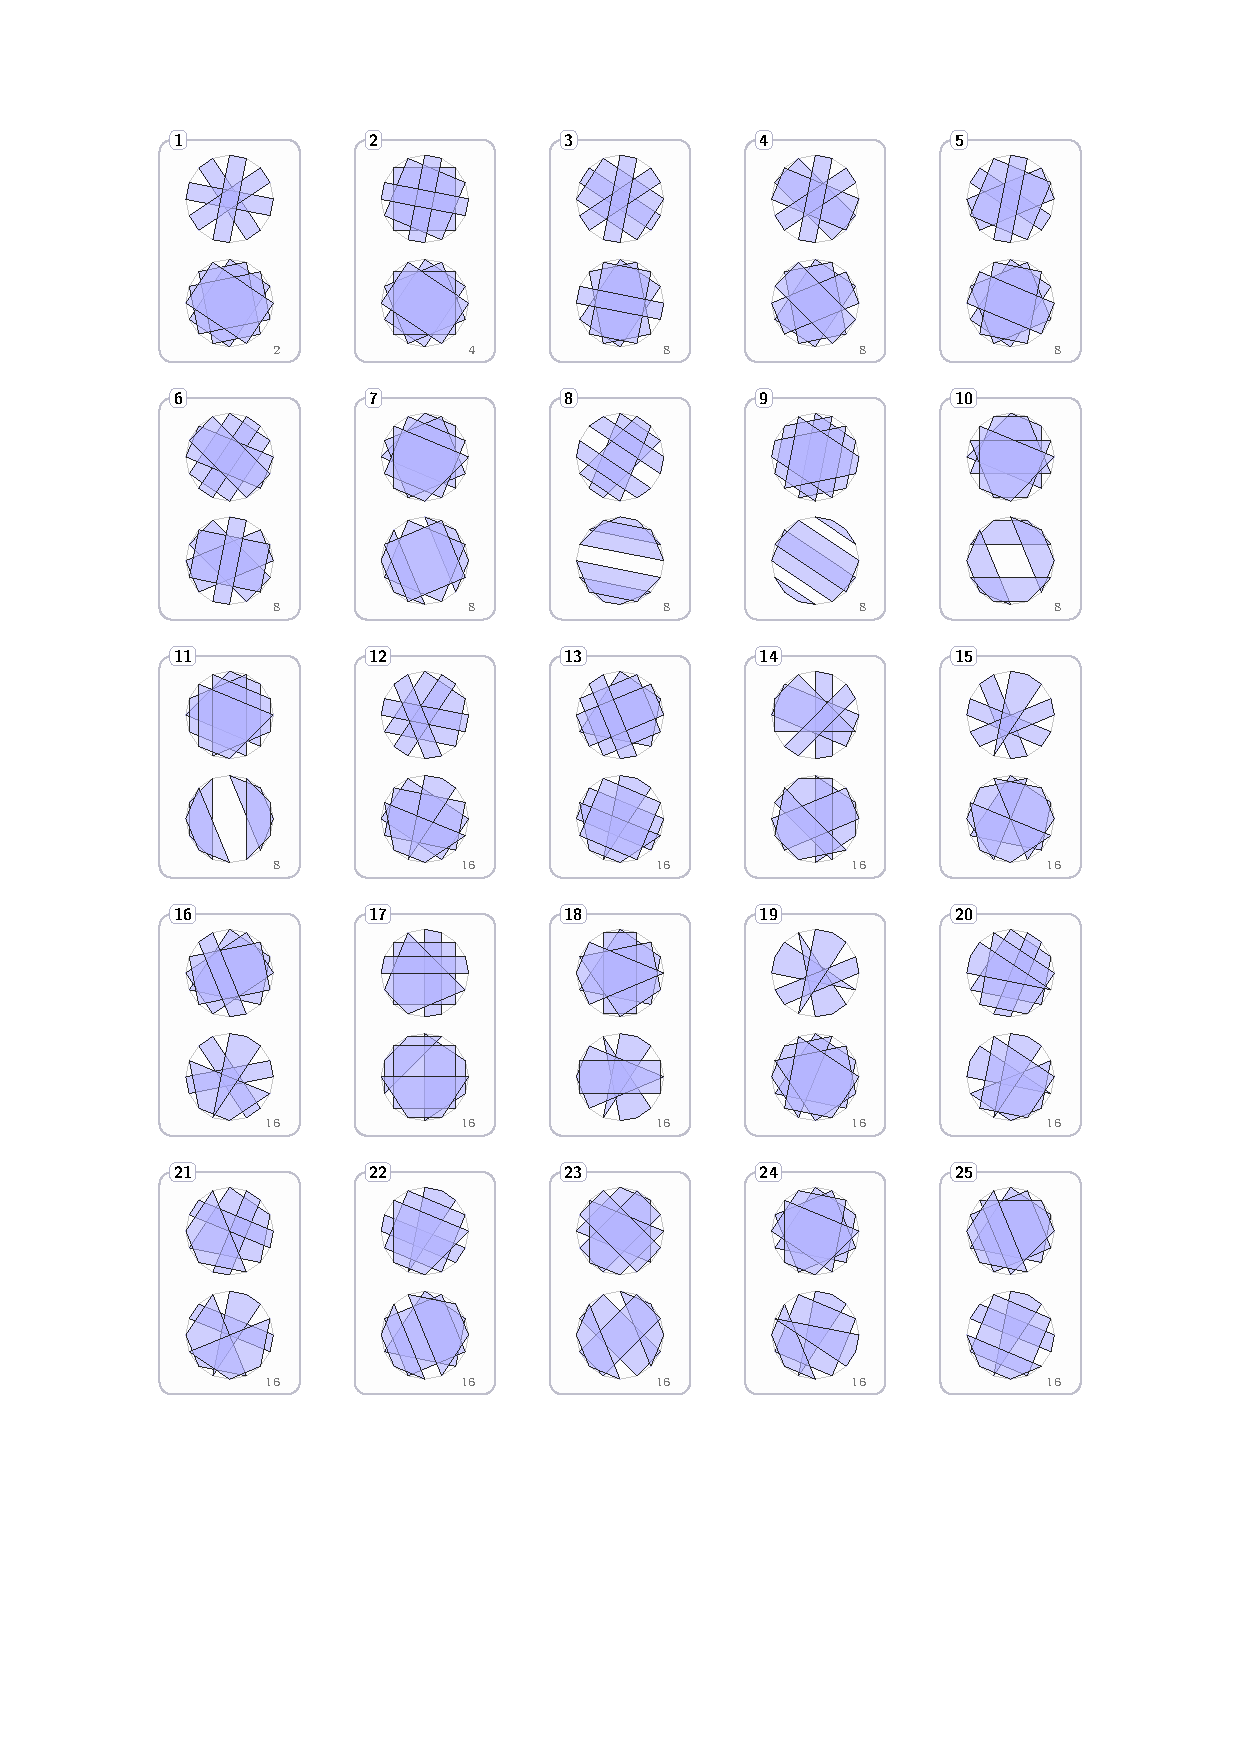
\includepdf[pages=-, pagecommand={\thispagestyle{headings}}]{plates/dimers_atlas.pdf}
